\section{Les tris}
%\leconwithtoc

\subsection{Objectif}

\begin{frame}
	voyons quelques algorithmes simples pour trier un
		ensemble d'informations~: recherche des maxima, tri
		par insertion et tri bulle dans un tableau. 
		Des algorithmes plus efficaces seront vus
		en deuxième année.
\end{frame}

\subsection{Motivation}

\begin{frame}{Motivation}
	Une application importante de l’informatique est le tri d’informations.
	La conception d’algorithmes efficaces pour ce type de traitement s’est
	imposée avec l’apparition de bases de données de taille importante. On
	citera par exemple la recherche d’un numéro de téléphone ou une adresse
	dans la version informatisée des pages blanches, ou de façon plus
	spectaculaire l’efficacité de certains moteurs de recherche qui
	permettent de retrouver en quelques secondes des mots clés arbitraires
	parmi plusieurs millions de pages sur le web.
\end{frame}

\begin{frame}{Motivation}
La recherche efficace d’information implique un tri préalable de
	celle-ci. En effet, si les données ne sont pas classées ou triées, le
	seul algorithme possible reviendrait à parcourir entièrement l’ensemble
	des informations. Pour exemple, il suffit d’imaginer un dictionnaire
	dans lequel les mots seraient mélangés de façon aléatoire au lieu
	d’être classés par ordre alphabétique. Pour trouver le moindre mot dans
	ce dictionnaire, il faudrait à chaque fois le parcourir entièrement !
	Il est clair que le classement préalable (ordre alphabétique) accélère
	grandement la recherche.
\end{frame}

\begin{frame}{Motivation}
	Ainsi, recherche et tri sont étroitement liés, et la façon dont les
	informations sont triées conditionne bien entendu la façon de
	rechercher l’information (cf. algorithme de recherche dichotomique).
	Pour exemple, prenons cette fois-ci un dictionnaire des mots croisés
	dans lequel les mots sont d’abord regroupés selon leur longueur et
	ensuite par ordre alphabétique. La façon de rechercher un mot dans ce
	dictionnaire est bien sûr différente de la recherche dans un
	dictionnaire usuel. 
\end{frame}

\begin{frame}{Motivation}
	Le problème central est donc le tri des informations. 
	
	\bigskip
	
	Celui-ci a pour
	but d’organiser un ensemble d’informations qui ne l’est pas \textit{à
	priori}. 
	
	\bigskip
	
	On peut distinguer trois grands cas de figure~:
\end{frame}

\begin{frame}{Motivation}
	\begin{itemize}
		\item 
			D’abord les situations impliquant le classement total d’un ensemble de
			données «~brutes~», c’est-à-dire complètement désordonnées. Prenons
			pour exemple les feuilles récoltées en vrac à l’issue d’un examen ; il
			y a peu de chances que celles-ci soient remises à l’examinateur de
			manière ordonnée ; celui-ci devra donc procéder au tri de l’ensemble
			des copies, par exemple par ordre alphabétique des noms des étudiants,
			ou par numéro de groupe etc.
	\end{itemize}
\end{frame}
	
\begin{frame}{Motivation}
	\begin{itemize}
		\item 
			Ensuite les situations où on s’arrange pour ne jamais devoir trier la
			totalité des éléments d’un ensemble, qui resterait cependant à tout
			moment ordonné. Imaginons le cas d’une bibliothèque~dont les livres
			sont rangés par ordre alphabétique des auteurs~: à l’achat d’un nouveau
			livre, ou au retour de prêt d’un livre, celui-ci est immédiatement
			rangé à la bonne place. Ainsi, l’ordre global de la bibliothèque est
			maintenu par la répétition d’une seule opération élémentaire consistant
			à insérer à la bonne place un livre parmi la collection. C’est la
			situation que nous considérerions dans le cas d'une structure
			où les éléments sont ordonnés.
	\end{itemize}
\end{frame}
	
\begin{frame}{Motivation}
	\begin{itemize}
		\item 
			Enfin, les situations qui consistent à devoir re-trier des données
			préalablement ordonnées sur un autre critère. Prenons l’exemple d’un
			paquet de copies d’examen déjà triées sur l’ordre alphabétique des noms
			des étudiants, et qu’on veut re-trier cette fois-ci sur les numéros de
			groupe. Il est clair qu’une méthode efficace veillera à conserver
			l’ordre alphabétique déjà présent dans la première situation afin que
			les copies apparaissent dans cet ordre dans chacun des groupes.
	\end{itemize}
\end{frame}
	
\begin{frame}{Motivation}
		Le dernier cas illustre un classement sur une \textbf{clé complexe}
	(ou \textbf{composée}) impliquant la comparaison de plusieurs champs
	d’une même structure~: le premier classement se fait sur le numéro de
	groupe, et à numéro de groupe égal, l’ordre se départage sur le nom de
	l’étudiant. On dira de cet ensemble qu’il est classé en \textbf{majeur}
	sur le numéro de groupe et en \textbf{mineur} sur le nom d’étudiant.
\end{frame}

\begin{frame}{Motivation}
		Notons que certains tris sont dits \textbf{stables} parce
	qu'en cas de tri sur une nouvelle clé, l’ordre de la
	clé précédente est préservé pour des valeurs identiques de la nouvelle
	clé, ce qui évite de faire des comparaisons sur les deux champs à la
	fois. Les méthodes nommées \textbf{tri par insertion}, \textbf{tri
	bulle} et \textbf{tri par recherche de minima successifs }(que nous
	allons aborder dans ce chapitre) sont stables.
\end{frame}

\begin{frame}{Motivation}
	Le tri d’un ensemble d’informations n’offre que des avantages. Outre le
	fait déjà mentionné de permettre une recherche et une obtention rapide
	de l’information, il permet aussi l’application de traitements
	algorithmiques efficaces (comme par exemple celui des ruptures que nous
	verrons plus loin) qui s’avéreraient trop coûteux (en temps, donc en
	argent !) s’ils s’effectuaient sur des ensembles non triés.
\end{frame}

\begin{frame}{Motivation}
	Certains tris sont évidemment plus performants que d’autres. Le choix
	d’un tri particulier dépend de la taille de l’ensemble à trier et de la
	manière dont il se présente, c’est-à-dire déjà plus ou moins ordonné.
	La performance quant à elle se juge sur deux critères~: le nombre de
	tests effectués (comparaisons de valeurs) et le nombre de transferts de
	valeurs réalisés. 
\end{frame}

\begin{frame}{Motivation}
	Dans ce chapitre, les algorithmes traiteront du tri dans un
	\textbf{tableau d’entiers à une }\textbf{dimension}. Toute autre
	situation peut bien entendu se ramener à celle-ci moyennant la
	définition de la relation d’ordre propre au type de données utilisé. Ce
	sera par exemple, l’ordre alphabétique pour les chaines de caractères,
	l’ordre chronologique pour des objets \textit{Date} ou
	\textit{Moment} (que nous verrons
	plus tard), etc. De plus, le seul ordre envisagé sera l’ordre
	\textbf{croissant} des données. Plus loin, on envisagera le tri 
	d'autres structures de données.
\end{frame}

\begin{frame}{Motivation}
	Enfin, dans toutes les méthodes de tri abordées, nous supposerons la
	taille physique du tableau à trier (notée $n$) égale à sa taille
	logique, celle-ci n’étant pas modifiée par l’action de tri.
\end{frame}

\subsection{Tri par insertion}

\begin{frame}{Tri par insertion}
	Cette méthode de tri repose sur le principe d’insertion de valeurs dans
	un tableau ordonné. 
\end{frame}

\begin{frame}{Tri par insertion}
	Le tableau à trier sera à chaque étape subdivisé en deux sous-tableaux~:
	le premier cadré à gauche contiendra des éléments déjà ordonnés, et le
	second, cadré à droite, ceux qu’il reste à insérer dans le sous-tableau
	trié. Celui-ci verra sa taille s’accroitre au fur et à mesure des
	insertions, tandis que celle du sous-tableau des éléments non triés
	diminuera progressivement.
\end{frame}

\begin{frame}{Tri par insertion}
	Au départ de l’algorithme, le sous-tableau trié est le premier élément
	du tableau. Comme il ne possède qu’un seul élément, ce sous-tableau est
	donc bien ordonné ! Chaque étape consiste ensuite à prendre le premier
	élément du sous-tableau non trié et à l’insérer à la bonne place dans
	le sous-tableau trié.
\end{frame}

\begin{comment}
\begin{frame}{Tri par insertion}
	Prenons comme exemple un tableau \code{tab} de 20 entiers. 
	
	Au départ, le	sous-tableau trié est formé du premier élément, 
	\code{tab[1]} qui vaut 20~:

	\begin{center}
	\begin{tabular}{*{20}{>{\centering\sffamily\itshape\arraybackslash}m{0.47cm}}}
		 1 &
		 2 &
		 3 &
		 4 &
		 5 &
		 6 &
		 7 &
		 8 &
		 9 &
		 10 &
		 11 &
		 12 &
		 13 &
		 14 &
		 15 & 
		 16 &
		 17 &
		 18 &
		 19 &
		 20
		 \\
	\end{tabular}
\end{frame}
\end{comment}

\begin{frame}{Illustration}

	Montrons par un exemple comment le module
	\textit{{max3}}
	peut faire appel au module
	\textit{{max2}}~:

	\bigskip
	
	\cadre{
	\begin{pseudo}
	\LComment Lit trois nombres et affiche le maximum des trois.
	\Module{max3}{}{}
		\Decl a, b, c, temp, max~: réels
		\Read a, b, c
		\Stmt max2( a, b, temp )
		\Stmt max2( temp, c, max )
		\Write max
	\EndModule
	\end{pseudo}
	}
\end{frame}

\begin{frame}{Illustration}
	
	L’instruction
	\textit{{max2(a, b,
	temp)}} se déroule comme suit~:
	
	\begin{itemize}
	\item {
	{le contenu des variables
	}\textit{{a}}{
	et
	}\textit{{b}}{
	est affecté aux paramètres d’entrée
	}\textit{{a}}{
	et
	}\textit{{b}}{
	du module
	}\textit{{max2}}{,
	puis ce module peut entrer en action~;}}
	\item {
	{à l’issue du module
	}\textit{{max2}}{,
	la valeur du paramètre de sortie
	}\textit{{max}}{
	est communiquée à la variable
	}\textit{{temp}}{,
	qui contient à présent le maximum de
	}\textit{{a}}{
	et
	}\textit{{b}}{.}}
	\end{itemize}
\end{frame}

\begin{frame}{Illustration}
	
	L’instruction \textit{max2(temp, c, max)}
	se déroule comme suit~:
	
	\begin{itemize}
	\item {
	{le contenu des variables
	}\textit{{temp}}{
	et
	}\textit{{c}}{
	est affecté aux paramètres d’entrée
	}\textit{{a}}{
	et
	}\textit{{b}}{
	du module
	}\textit{{max2}}{,
	puis ce module peut entrer en action~;}}
	\item {
	{à l’issue du module
	}\textit{{max2}}{,
	la valeur du paramètre de sortie
	}\textit{{max}}{
	est communiquée à la variable
	}\textit{{max}}{,
	qui contient à présent le maximum des 3 nombres de départ.}}
	\end{itemize}

	{Il est évident que la présence de ces deux
	instructions dans le module
	}\textit{{max3}}{
	implique la présence du module
	}\textit{{max2}}{
	«~aux alentours~» du premier, c’est-à-dire que ces deux modules doivent
	se trouver sur le même support d’écriture de
	l'algorithme complet.}
\end{frame}

\begin{frame}{Remarques}
	\begin{itemize}
	\item {
	{un paramètre peut être à la fois paramètre
	d’entrée et de sortie~; on le fait suivre alors de la double flèche
	}{$\uparrow \downarrow$}{~;}}
	\item {
	si tous les paramètres sont en entrée, on peut omettre les flèches;}
	\item {
	la présence de ces paramètres n’est pas obligatoire, on peut envisager
	un module sans paramètre de sortie (par ex. un module qui reçoit en
	entrée un nombre et dont la seule fonction est de l’afficher à
	l’écran), ou inversement sans paramètre d’entrée (un module qui simule
	un lancer de dé, et renvoie en paramètre une valeur aléatoire entre 1
	et 6)~;}
	\end{itemize}
\end{frame}

\begin{frame}{Remarques}
	\begin{itemize}
	\item {
	{pour appeler correctement un module, il faut
	fournir des noms de variables, des expressions ou des constantes
	}{\textbf{en même
	nombre}}{ et en même ordre que les paramètres
	du module~;}}
	\item {
	en outre, les types des variables doivent correspondre entre l’appel et
	l’en-tête du module~;}
	\item {
	ne peut être affectée à un paramètre d’entrée du module qu’une
	constante, une expression ou une variable préalablement affectée~;}
	\end{itemize}
\end{frame}

\begin{frame}{Remarques}
	\begin{itemize}
	\item {
	à un paramètre de sortie d’un module doit toujours correspondre une
	autre variable, jamais une constante ou une expression~;}
	\item {
	il faut s’assurer qu’à l’issue du module, tous les paramètres de sortie
	aient été affectés lors de l’exécution de ce module.}
	\end{itemize}

\end{frame}

\subsection{Variables locales}

\begin{frame}{variables locales}
	\begin{itemize}
	\item
	Dans le cadre de ce cours d’algorithmique,
	nous n’envisagerons que l’utilisation de 
	\textbf{variables locales}. 
	\item
	Toute variable est \textbf{locale} au module 
	dans lequel elle apparait, ce qui veut dire que son existence
	est ignorée en dehors de ce module. 
	\item
	Nous n’envisageons donc pas ici l’utilisation déconseillée de 
	\textbf{variables globales} 
	(variables dont le contenu est reconnu 
	par tous les modules d’un programme).
	\item
	Précisons qu'une variable locale est aussi
	\textbf{dynamique}, c’est-à-dire qu’un emplacement en mémoire lui est
	réservé durant l’exécution du module où elle est déclarée. Une fois
	l’exécution terminée, cet emplacement est récupéré en mémoire.
	\end{itemize}
\end{frame}

\begin{frame}{variables locales}
	\begin{itemize}
	\item
	Plutôt qu’une restriction, cette propriété est
	une aide confortable au programmeur~: si, de
	façon fortuite, des variables appartenant à des modules différents
	possédaient le même nom, il n’y aurait pas d’interférence entre ces
	variables, ni confusion possible de leur
	contenu.
	\item
	Notons au passage que les variables déclarées dans l’entête du module ne
	doivent plus l’être dans la partie «~déclaration de variables~» de ce
	module. Mais toutes les variables utilisées dans un module doivent être
	déclarées, soit dans son entête, soit dans sa déclaration. Le
	non-respect de cette règle provoquerait une erreur d’exécution.
	\end{itemize}
\end{frame}

\begin{frame}{exemple}
	\cadre{
	\begin{pseudo}
	\LComment Lit trois nombres positifs et affiche le maximum des trois.
	\Module{max3}{}{}
		\Decl a, b, c, temp, max~: réels
		\Stmt lirePositif(a)
		\Stmt lirePositif(b)
		\Stmt lirePositif(c)
		\Stmt max2(a, b, temp)
		\Stmt max2(temp, c, max)
		\Write max
	\EndModule
	\end{pseudo}
	}
\end{frame}

\begin{frame}{exemple}
	\cadre{
	\begin{pseudo}
	\LComment Lit un nombre, le sort s'il est positif et sinon lance une erreur.
	\Module{lirePositif}{a\Out~: réel}{}
		\Read a
		\If{a < 0}
			\Error Le nombre n'est pas positif !
		\EndIf
	\EndModule
	\end{pseudo}
	}
\end{frame}

\begin{frame}{exemple}
	\cadre{
	\begin{pseudo}
	\LComment Affiche deux nombres et sort le maximum des deux.
	\Module{max2}{a\In, b\In~: réels, max\Out~: réel}{}
		\If{a > b}
			\Let max \Gets a
		\Else
			\Let max \Gets b
		\EndIf
	\EndModule
	\end{pseudo}
	}
\end{frame}

\subsection{Module renvoyant une valeur}

\begin{frame}{valeur en retour}
	Un deuxième type de module est le 
	\textbf{module renvoyant une valeur}. 
	
	(On désigne aussi ce type de modules par le terme \textbf{fonction}).
	
	\bigskip
	
	Son entête est du type suivant~:

	\bigskip
	
	\cadre{
	\begin{pseudo}
	\ModuleSign{exemple }{var1\In~: type1, var2\In~: type2, \dots, varN\In~: typeN}{typeRes}
	\end{pseudo}
	}
\end{frame}

\begin{frame}{valeur en retour}
	Il se distingue du module précédemment étudié par la flèche de renvoi à
	droite, et possède les particularités suivantes~:

	\begin{itemize}
	\item {
		{ce module renvoie
		}{\textbf{une}}{
		}{\textbf{valeur}}{
		}{\textbf{qui n’est pas affectée à une variable
		de
		}}{\textbf{sortie~}}{;}}
	\item {
		{à droite de la flèche de renvoi ne se trouve
		donc pas le nom d’un paramètre de sortie, mais le
		}{\textbf{type}}{ de la
		valeur renvoyée~;}}
	\item {
		\textit{{typeRes}}{
		est le type de la valeur renvoyée~; 
		
		en théorie, ce peut être 
		\begin{itemize}
		\item
		un type
		simple (entier, réel, booléen, chaine, caractère), 
		\item
		un type structuré,
		\item
		un tableau 
		\item
		ou même un objet (ces types seront vus dans les chapitres 
		suivants). 
		\end{itemize}
		En pratique il conviendra de s’en tenir aux limitations 
		du langage utilisé~;}}
	\end{itemize}
\end{frame}

\begin{frame}{valeur en retour}
	\begin{itemize}
	\item {
		\textit{{var1}}{,
		...,
		}\textit{{varN}}{
		sont les paramètres du module (aussi appelés
		}{\textbf{arguments}}{)
		; ce sont, le plus souvent, des paramètres d’entrée, les paramètres de
		sortie }{étant plus rares dans ce type de
		module~;}}
	\item {
		ces arguments deviennent automatiquement des variables locales du module
		; déclarées dans son en-tête, elles ne doivent plus l’être dans la
		partie déclarative~;}
		\end{itemize}
\end{frame}

\begin{frame}{valeur en retour}
	\begin{itemize}
	\item {
		{la valeur renvoyée est définie à la fin du
		module via la primitive
		}\textit{{retourner}}{
		}\textit{{résultat}}{,
		où
		}\textit{{résultat}}{
		est une variable (ou plus généralement une expression) de type
		}\textit{{typeRes}}{
		;}}
	\item {
		pour appeler ce type de module, on utilise son nom \textit{comme celui
		d’une variable} ou dans une expression apparaissant 
		dans le module appelant, mais jamais à gauche du signe
		d’affectation.}
	\end{itemize}
	
	\bigskip
	
	Comme précédemment, il faut veiller, lors de l’appel de ce 
	type de module, à ce que le nombre d’arguments ainsi que leur type
	correspondent à ceux spécifiés dans l’entête.
\end{frame}

\begin{frame}{exemple}
	Pour exemple, transformons une fois de plus la
	dernière version de notre algorithme.
	
	\bigskip
	
	\cadre{
	\begin{pseudo}
	\LComment Lit trois nombres positifs et affiche le maximum des trois.
	\Module{max3}{}{}
		\Decl a, b, c, temp, max~: réels
		\Let a \Gets lirePositif()
		\Let b \Gets lirePositif()
		\Let c \Gets lirePositif()
		\Let temp \Gets max2(a, b)
		\Let max  \Gets max2(temp, c)
		\Write max
	\EndModule
	\end{pseudo}
	}
\end{frame}

\begin{frame}{exemple}
	\cadre{
	\begin{pseudo}
	\LComment Lit un nombre, le retourne s'il est positif et sinon lance une erreur.
	\Module{lirePositif}{}{réel}
		\Decl a~: réel
		\Read a
		\If{a < 0}
			\Error Le nombre n'est pas positif !
		\EndIf
		\Return a
	\EndModule
	\end{pseudo}
	}
\end{frame}

\begin{frame}{exemple}
	\cadre{
	\begin{pseudo}
	\LComment Affiche deux nombres et retourne le maximum des deux.
	\Module{max2}{a\In, b\In~: réels}{réel}
		\Decl max~: réel
		\If{a > b}
			\Let max \Gets a
		\Else
			\Let max \Gets b
		\EndIf
		\Return max
	\EndModule
	\end{pseudo}
	}
\end{frame}

\begin{frame}{exemple}
	L'écriture avec une valeur de retour permet une
	écriture plus compacte~:

	\bigskip
	
	\cadre{
	\begin{pseudo}
	\LComment Lit trois nombres positifs et affiche le maximum des trois.
	\Module{max3}{}{}
		\Decl a, b, c, max~: réels
		\Let a \Gets lirePositif()
		\Let b \Gets lirePositif()
		\Let c \Gets lirePositif()
		\Let max  \Gets max2(max2(a, b), c)
		\Write max
	\EndModule
	\end{pseudo}
	}
\end{frame}

	\bigskip
	
\begin{frame}{exemple}
	ou encore (mais on perd un peu en clarté)~:

	\bigskip
	
	\cadre{
	\begin{pseudo}
	\LComment Lit trois nombres positifs et affiche le maximum des trois.
	\Module{max3}{}{}
		\Decl a, b, c~: réels
		\Let a \Gets lirePositif()
		\Let b \Gets lirePositif()
		\Let c \Gets lirePositif()
		\Write max2(max2(a, b), c)
	\EndModule
	\end{pseudo}
	}

	\bigskip
	
	ou même (et là, ce n'est plus du tout lisible !)~:

	\bigskip
	
	\cadre{
	\begin{pseudo}
	\LComment Lit trois nombres positifs et affiche le maximum des trois.
	\Module{max3}{}{}
		\Write max2(max2(lirePositif(), lirePositif()), lirePositif())
	\EndModule
	\end{pseudo}
	}
\end{frame}

\subsection{Un exemple complet}

\begin{frame}{Écart entre 2 moments}
	Étant donné deux moments dans une journée donnés chacun par trois
	nombres (heure, minute, seconde), 
	
	écrire un algorithme qui calcule et
	affiche le délai écoulé entre ces deux moments en heure(s), minute(s),
	seconde(s) 
	
	sachant que le deuxième moment donné est chronologiquement
	postérieur au premier.
\end{frame}

\begin{frame}{Écart entre 2 moments}
	Le problème n'est pas simple. 
	
	\bigskip
	
	On pourrait se dire qu'il suffit de soustraire les heures, 
	les minutes et les secondes.

	\bigskip
	
	Ainsi, pour l'écart entre
	1h22'23'' et
	3h34'56'', on
	calcule 3h-1h=2h;
	34'-22'=12' et
	56''-23''=33''
	ce qui donne un écart de
	2h12'33''.

	\bigskip
	
	Mais il s'agit là d'un cas favorable
	sans résultat négatif. 
	
	\bigskip
	
	Si une des soustractions est négative, comme par
	exemple pour l'écart entre
	1h22'23'' et
	3h11'12'', de
	simples soustractions ne suffisent pas.
\end{frame}

\begin{frame}{Écart entre 2 moments}
	Rappelons-nous que nous
	avons déjà écrit des algorithmes proches de ce problème dans les
	exercices du chapitre sur les algorithmes séquentiels. 
	
	\bigskip
	
	Plus précisément~:

	\bigskip
	
	\cadre{
	\begin{pseudo}
		\ModuleSign{heuresEnSecondes}{}{}
		\ModuleSign{secondesEnHeures}{}{}
	\end{pseudo}
	}
\end{frame}

\begin{frame}{Écart entre 2 moments}
	L'idée est de tout convertir en
	secondes car alors la soustraction est simple. 
	
	\bigskip
	
	Le résultat est alors
	reconverti en heures-minutes-secondes.

	\begin{center}
	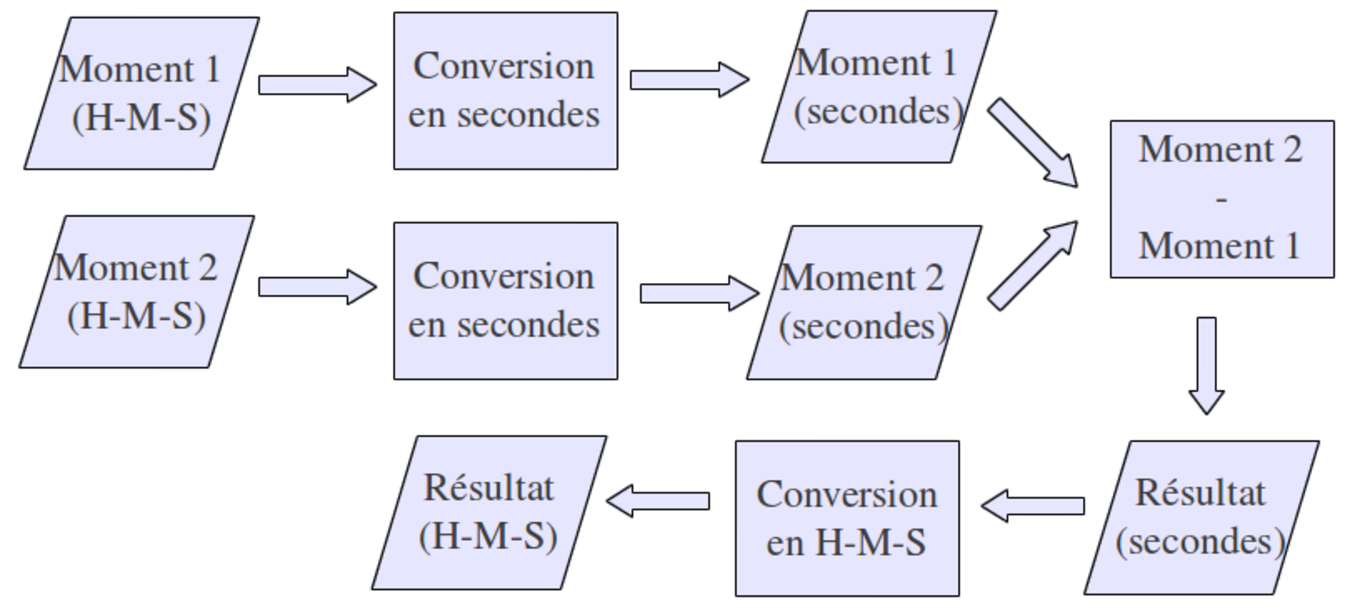
\includegraphics[width=0.8\textwidth]{image/module-conversion}
	\end{center}
\end{frame}

\subsubsection{Conversion en secondes}

\begin{frame}{Écart entre 2 moments}
	Une des sous-tâches est donc la conversion en secondes
	d'un moment exprimé en heures-minutes-secondes
	(h-m-s). 
	
	\bigskip
	
	Il nous faut adapter la solution trouvée pour
	l'exercice du chapitre sur les algorithmes séquentiels
	car il n'est pas question ici que les données soient
	lues ni que le résultat soit écrit~; 
	
	\bigskip
	
	l'interaction ne
	se fait pas avec l'utilisateur mais avec le module
	principal qui va l'utiliser.
\end{frame}

\begin{frame}{Écart entre 2 moments}
	La première question à se poser est donc celle des paramètres~:

	\bigskip
	
	\begin{itemize}
	\item 
		Quelles sont les données dont a besoin l'algorithme
		pour travailler ?
	\item 
		Quels résultats fournit-il ?
	\end{itemize}
\end{frame}

\begin{frame}{Écart entre 2 moments}
	Dans notre cas, la réponse est simple~:

	\bigskip
	
	\begin{itemize}
	\item {
		Les données sont le moment à convertir en secondes. 
		
		Ce moment est
		représenté par trois entiers~: les heures, les minutes et les secondes
		;}
	\item {
		Le résultat est le moment converti en secondes. 
		
		Il est représenté par un entier.}
	\end{itemize}
\end{frame}

\begin{frame}{Écart entre 2 moments}
	Lorsque le résultat est représenté par une seule donnée, on a le choix
	entre un paramètre en sortie~:

	\bigskip
	
	\cadre{
	\begin{pseudo}
		\LComment Affiche trois entiers~: des heures, des minutes et des secondes et sort le nombre de secondes correspondant.
		\ModuleSign{hmsVersSec}{h\In, m\In, s\In, secondes\Out~: entiers}{}
	\end{pseudo}
	}
	
	\bigskip
	
	ou une valeur de retour~:

	\bigskip
	
	\cadre{
	\begin{pseudo}
		\LComment Affiche trois entiers~: des heures, des minutes et des secondes et retourne le nombre de secondes correspondant.
		\ModuleSign{hmsVersSec}{h\In, m\In, s\In~: entiers}{entier}
	\end{pseudo}
	}
\end{frame}

\begin{frame}{Écart entre 2 moments}
		Dans de pareils cas, 
	on privilégie souvent la valeur de retour car cela
	facilite l'écriture lors de l'appel.

	\bigskip
	
	L'algorithme s'écrit alors~:

	\bigskip
	
	\cadre{
	\begin{pseudo}
	\LComment Affiche trois entiers~: des heures, des minutes et des secondes 
	\LComment et retourne le nombre de secondes correspondant.
		\Module{hmsVersSec}{h\In, m\In, s\In~: entiers}{entier}
			\Decl secondes~: entier \RComment {À déclarer puisque ce n'est pas un paramètre}
			\Let secondes \Gets  h * 3600 + m * 60 + s
			\Return secondes
		\EndModule
	\end{pseudo}
	}
\end{frame}

\begin{frame}{Écart entre 2 moments}
	ou de manière équivalente mais plus concise~:

	\bigskip
	
	\cadre{
	\begin{pseudo}
	\LComment Affiche trois entiers~: des heures, des minutes et des secondes 
	\LComment et retourne le nombre de secondes correspondant.
		\Module{hmsVersSec}{h\In, m\In, s\In~: entiers}{entier}
			\Return h * 3600 + m * 60 + s
		\EndModule
	\end{pseudo}
	}
\end{frame}

\subsubsection{Conversion en heures-minutes-secondes}

\begin{frame}{Conversion en heures-minutes-secondes}
	À la fin de notre algorithme, il nous faudra reconvertir un résultat
	exprimé en secondes sous la forme heures-minutes-secondes. 
	
	\bigskip
	
	À nouveau,
	on a déjà résolu ce problème dans le chapitre sur les algorithmes
	séquentiels. 
	
	\bigskip
	
	Mais il faut l'adapter à
	l'usage de paramètres.
\end{frame}

\begin{frame}{Conversion en heures-minutes-secondes}
	\begin{itemize}
	\item {
		Quelles sont les données ? 
		
		Une seule, le moment exprimé en secondes}
		
	\bigskip
	
	\item {
		Quels sont les résultats calculés par le module ? 
		
		Ce même moment exprimé
		en heures-minutes-secondes. 
		
		Trois entiers sont requis ce qui fait que
		le choix entre un paramètre en sortie et une valeur de retour ne se
		pose pas ici~; 
		
		impossible d'utiliser une valeur de
		retour (qui doit être unique)~; 
		
		on doit utiliser des paramètres en
		sortie.}
	\end{itemize}
\end{frame}

\begin{frame}{Conversion en heures-minutes-secondes}
	Ce qui donne~:

	\bigskip
	
	\cadre{
	\begin{pseudo}
		\LComment Affiche un nombre de secondes et sort les heures, les minutes et les secondes correspondant.
		\Module{secVersHMS}{secondes\In, s\Out, m\Out, s\Out~: entiers}{}
			\Let h \Gets secondes DIV 3600
			\Let m \Gets (secondes MOD 3600) DIV 60
			\Let s \Gets secondes MOD 60
		\EndModule
	\end{pseudo}
	}
\end{frame}

\subsubsection{Solution}

\begin{frame}{Solution}
	À présent, on a tout pour écrire la solution à notre problème

	\bigskip
	
	\cadre{
	\begin{pseudo}
		\LComment Lit deux moments (h-m-s) et affiche le moment de la différence entre les deux.
		\Module{différenceEntreHeures}{}{} \RComment Pas de paramètres !
			\Decl h1, m1, s1, h2, m2, s2~: entiers \RComment Les 2 moments à soustraire
			\Decl secondes1, secondes2~: entiers \RComment Ces 2 moments en secondes
			\Decl diffSecondes~: entier \RComment La différence en secondes
			\Decl diffH, diffM, diffS~: entiers \RComment La différence en H-M-S
			\Read h1, m1, s1, h2, m2, s2
			\Let secondes1 \Gets hmsVersSec( h1, m1, s1 )
			\Let secondes2 \Gets hmsVersSec( h2, m2, s2 )
			\Let diffSecondes \Gets secondes2 – secondes1
			\Stmt secVersHMS( diffSecondes, diffH, diffM, diffS )
			\Write diffH, diffM, diffS
		\EndModule
	\end{pseudo}
	}
\end{frame}

\begin{frame}{Solution}
	Dans la solution ci-dessus, 
	quelle est ou quelles sont la/les variable(s) locale(s) 
	dont on pourrait se passer moyennant une réécriture de
	l'algorithme ?
\end{frame}

\subsection{Blocs}

\begin{frame}{Blocs}
	\begin{itemize}
	\item
	Un bloc est l’écriture d’une portion de module
	à l’extérieur de celui-ci. C’est un simple
	{\textit{déplacement}}
	de lignes de codes vers un autre endroit du texte de
	l'algorithme.
	
	\bigskip
	
	\item
	La raison de découper un module en blocs
	peut être le souci de clarifier un algorithme en le découpant en étapes
	bien distinctes.
	
	\bigskip
	
	\item
	Les variables
	d’un bloc ne sont donc pas des variables locales du bloc dans lequel
	elles apparaissent, mais bien des variables locales du module auquel
	appartient ce bloc.
	\end{itemize}
\end{frame}

\begin{frame}{Blocs}
	\begin{itemize}
	\item
	L’appel de l’exécution des instructions se trouvant
	dans un bloc est similaire à celui d’un module avec paramètres, on
	écrit simplement le nom du bloc comme s’il s’agissait d’une
	instruction.
	\end{itemize}
\end{frame}

\begin{frame}{Blocs}
	Pour exemple, le module additionnerFractions (première version dans le
	chapitre 3) pourrait se découper ainsi~:

	\bigskip
	
	\cadre{
	\begin{pseudo}
	\LComment Lit les contenus de 2 fractions et affiche leur somme
		\Module{additionnerFractions}{}{}
			\Stmt déclaration
			\Stmt lectureDonnées
			\Stmt calculs
			\Stmt écritureRésultat
		\EndModule
	\end{pseudo}
	}
\end{frame}

\begin{frame}{Blocs}
	\cadre{
	\begin{pseudo}
	\Block{déclaration}
		\Decl num1, den1, num2, den2, numRes, denRes~: entiers
	\EndBlock
	\end{pseudo}
	}

	\bigskip
	
	\cadre{
	\begin{pseudo}
	\Block{lectureDonnées}
		\Read num1, den1, num2, den2
	\EndBlock
	\end{pseudo}
	}
\end{frame}

\begin{frame}{Blocs}
	\cadre{
	\begin{pseudo}
	\Block{calculs}
		\Let numRes \Gets num1 * den2 + num2 * den1
		\Let denRes \Gets den1 * den2
	\EndBlock
	\end{pseudo}
	}

	\bigskip
	
	\cadre{
	\begin{pseudo}
	\Block{écritureRésultat}
		\Write numRes, "/", denRes \RComment la fraction n'est pas simplifiée
	\EndBlock
	\end{pseudo}
	}
\end{frame}

\subsection{Qu'est-ce qu'un algorithme de qualité ?}

\begin{frame}{Algorithme de qualité}
	\begin{itemize}
	\item
	Nous voulons tous produire du code de qualité mais
	qu'est-ce que cette notion recouvre vraiment ?
	\item
	Qu'est-ce qui permet de juger de la qualité
	d'un code ? 
	\item
	De nombreux critères existent. 
	\end{itemize}
	
	\bigskip
	
	Citons ici,
	parmi les plus pertinents, ceux qui sont le plus liés à ce
	cours.
\end{frame}

\begin{frame}{Algorithme de qualité}
	\begin{itemize}
	\item
		La \textbf{validité}~: le code doit
	réaliser les tâches pour lesquelles 
	il a été écrit, même dans tous les
	cas particuliers imaginés.
	
	\bigskip
	
	\item 
		L'\textbf{extensibilité} (ou évolutivité)~:
	le code doit être écrit de telle sorte qu'un changement
	mineur dans le problème n'implique
	qu'un changement mineur dans le code.
	
	\bigskip
	
	\item
		La \textbf{réutilisabilité}~: c'est
	la capacité de réutiliser 
	un bout de code d’un projet dans un autre projet de 
	façon aisée et sûre.
	\end{itemize}
\end{frame}

\begin{frame}{Algorithme de qualité}
	\begin{itemize}
	\item
		La \textbf{lisibilité}~: 
		
	Au niveau global, on doit facilement comprendre la structure
	générale du code afin de pouvoir aisément comprendre où se trouve 
	la portion de	code qui nous intéresse. 
	
	Au niveau local, on doit pouvoir comprendre
	aisément chaque bout de code.
	
	\bigskip
	
	\item 
		L'\textbf{efficience}~: 
	ce critère s'intéresse à la bonne utilisation des
	ressources informatiques. Est-ce que le programme va tourner
	suffisamment vite, utiliser peu de mémoire ?
	\end{itemize}
\end{frame}
